\section{Siamese Multi-Object Tracking and ReID}
\label{sec:SiamMOTandReID}

% ##############################################################################
\subsection{Motivation}

The use of \gls{reid} has been emphasized numerous times during our preliminary research for this thesis. We conjectured that once full occlusion ensues, the \gls{reid} mechanism could be adopted to recover the lost track since the object appears at the scene as a new one. The presence of occlusion percolates traffic scenes, especially if the camera does not view the road from a higher position. At the beginning of our Ph.D. research, we worked on the \interreg{} project where we tackled vehicle tracking when the camera was positioned next to the road (\figtext{}~\ref{fig:InterregDatasetSample}). Under these circumstances, occlusion was inevitable. Such a setup inexorably led to situations in which a vehicle appeared for a second on the left side of the frame, then ended up fully covered by a truck, and re-appeared for a miniscule amount of time at the other side of frame. The task of maintaining the same object identifier was burdensome and often impossible with high degree of precision.

% ##############################################################################
\subsection{Preliminary Discussion}

To make a full disclosure right at the beginning, we expected that the adoption of \gls{reid} enhancements within the \gls{siammot} framework would bring improvements in certain areas. Retrospectively, our experiments showed detrimental effects upon the tracker accuracy. Despite our negative outcome, we still consider the performed research to be a contribution to the \gls{mot} area. We will elaborate further on why it is so in order to learn from such an experience as much as possible. Our surprise stems primarily from the fact that our thesis goals revolved around the application of \gls{reid} in object tracking. Therefore, finding that such approach does not yield the desired outcome raises multiple questions, specifically the following ones:
\begin{enumerate}
    \item Does the inclusion of \gls{reid} into \gls{mot} frameworks have a potential to resolve cases of full occlusion without exacerbating other areas?
    \item Is the \gls{reid} extension suitable to the chosen \gls{mot} model, namely, the \gls{siammot}?
    \item Is the target use case in terms of datasets adequate to showcase the potential of \gls{reid} applied in the \gls{siammot} tracker?
\end{enumerate}

% ##############################################################################
\subsection{Proposed ReID-Enhanced Architecture}
\label{ssec:ProposedReIDEnhancedArchitecture}

We adopted the object \gls{reid} approach published in~\cite{luo2019bagoftricksreid}, a simple yet very robust framework for person \gls{reid}. We employed this architecture (\figtext{}~\ref{fig:BagOfTricksReIDArchitecture}) for vehicle \gls{reid} due to its simplicity accompanied with \gls{sota} performance at the time of publishing.

% ------------------------------------------------------------------------------
\begin{figure}[!t]
    \centering
    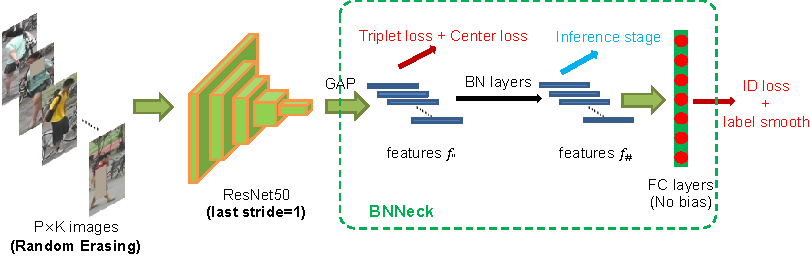
\includegraphics[width=\linewidth]{figures/siamese_tracking/bagoftricks_reid_architecture.pdf}
    \caption[Gls{reid} baseline]{A object \gls{reid} baseline which we used for our experiments. \externalsrc{\cite{luo2019bagoftricksreid}}}
    \label{fig:BagOfTricksReIDArchitecture}
\end{figure}
% ------------------------------------------------------------------------------

% ##############################################################################
\subsection{Training Phase}

Since this experiment was the first one we embarked upon, we tried to avoid modifications to the underlying tracker framework. Only upon obtaining prospective tracking improvements we would consider incorporating the object \gls{reid} into the whole end-to-end pipeline. As a result, the \gls{siammot} training phase was not modified. We employed an external object \gls{reid} network to perform embedding computation during the inference phase. As far as the training of the \gls{reid} network is concerned, we adopted a standard approach of using the triplet loss (\eqtext{}~\ref{eq:TripletLoss} on page \pageref{eq:TripletLoss}) in conjunction with the categorical cross-entropy loss for additional learning signal. We trained the model using the \verisss{} dataset on which the evaluation was performed, too. The model was trained to produce $l_2$-normalized embedding vectors that were then used to measure the degree of similarity between vehicles.

% ##############################################################################
\subsection{Inference Phase}

The online solver algorithm was, from our point of view, the primary suspect for potential improvements due to its inherent simplicity that we considered inferior compared to the rest of the architecture. The aim was to adopt the already trained \gls{reid} model to help re-instantiate lost tracks due to occlusion. This external module would be invoked on demand, in a deterministic way as part of the online solver phase. At this stage of research we did strive for simplicity rather than efficiency. Consequently, the model inference was substantially impaired by a four-fold speed reduction as measured by \gls{fps}, because there was another independent model to process the input frame.

We isolated the modifications to the inference phase only within the online solver itself. Thus, we developed a whole new algorithm that handled the newly trained external model as well. The original processing steps of the online solver are outlines in \figtext{}~\ref{fig:SiamMOTOnlineSolver}. Our custom inference algorithm is described the pseudocode below.

\todo[inline]{Add pseudocode for the ``track solver + ReID'' solution.}

% ##############################################################################
\subsection{Experimental Evaluation and Discussion}

Due to the already excessive length of this document and inferior results this experiment brought in terms of tracking accuracy and inference speed, we decided to omit extensive documentation. There are more important experiments that deserve a deeper elaboration.

To say the least, we encountered several situations that indicated improvments. At certain occasions, the model was capable of properly identifying the lost object based on the embedding vector distance. However, such situations were relatively rare. What pulled the tracker's accuracy down was the detrimental effect of the \gls{reid} module during the \gls{nms} phase. The original online solver uses the \gls{nms} algorithm to assign detections to either active or dormant tracks. This phase is very effective and covers a great deal of common situations.

Our observations brought the following question. Is it more likely for the occluded object to appear at completely different position within the frame or somewhere near the position of disappearance? If we constraint ourselves to the \interreg{} project with the road viewed from the side (\figtext{}~\ref{fig:InterregDatasetSample}), then it might hold true most of the time. However, in general traffic analysis, especially in the scenes from the \uadetrac{} dataset, it is scarcely true. Vehicles often re-appear near the position where they last disappeared. As a result, the original online solver covered such situations very effectively. In fact, it even outperformed the entire \gls{reid} model due to its ability to assess the object similarity thanks to similarity learning. Remember that the search region commonly encompasses an area with sides of double length as compared to the exemplar region.

Another problem appears during partial occlusion. A vehicle is often severly occluded by another vehicle, so the two \glspl{bbox} enclose both objects. The embedding distances for the two objects are very close. In terms of the \gls{reid} mechanism, the two delineated regions given by the two \glspl{bbox} of closely positioned objects with severe occlusion are sometimes considered to be the same object. Consequently, the two tracks are merged into one.

\todo[inline]{Add image showing the situation of severe occlusion.}

We conjecture that the \gls{reid} is useful for multi-camera scenarios where the task is to re-identify the object from completely different angle, often without partial occlusion. In common crossroad situations which are abundant in the \uadetrac{} dataset, the first formulation of the online solver approach handles partial occlusion with a lot higher precision than our \gls{reid} extension.

This experiment showed that the inclusion of \gls{reid} mechanism into the inference algorithm brings a lot more disadvantages than benefits and we did not continue with this path.
